\documentclass{beamer}
%% fink install texlive
\usetheme{Warsaw}

\usepackage{amsmath,amssymb}
\usepackage{stmaryrd}
\usepackage{graphicx}
%\usepackage{haskell}
\usepackage{code}
%\usepackage{proof}
\usepackage{theorem}
\usepackage{pstricks} 
\usepackage{listings}
\usepackage{pgf-pie} % from https://code.google.com/p/pgf-pie/



% Martin's macros
   

% groups

%%\newtheorem{lemma}{Lemma}
%%\newtheorem{definition}{Definition}
%%\newtheorem{theorem}{Theorem}
%%\newtheorem{corollary}{Corollary}
%%\newtheorem{remark}{Remark}
%%\newtheorem{conjecture}{Conjecture}
%%\newtheorem{example}{Example}

% arrays

\newcommand{\bi}{\begin{array}[t]{@{}l@{}}}
\newcommand{\ei}{\end{array}}
\newcommand{\ba}{\begin{array}}
\newcommand{\ea}{\end{array}}
\newcommand{\bda}{\[\ba}
\newcommand{\eda}{\ea\]}
\newcommand{\bp}{\begin{quote}\tt\begin{tabbing}}
\newcommand{\ep}{\end{tabbing}\end{quote}}
\newcommand{\set}[1]{\left\{
    \begin{array}{l}#1
    \end{array}
  \right\}}
\newcommand{\sset}[2]{\left\{~#1 \left|
      \begin{array}{l}#2\end{array}
    \right.     \right\}}


% symbols

\newcommand{\good}{good}
 
\newcommand{\err}{{\bf W}}
\newcommand{\VV}{{\cal V}} 
\newcommand{\GT}{{\cal T}_G}
\newcommand{\KK}{{\cal K}}
\newcommand{\TT}{{\cal T}}
\newcommand{\TC}{\mbox{\it TC}}
\newcommand{\UL}{\mbox{UL}}
\newcommand{\sUL}{\mbox{\scriptsize UL}}
\newcommand{\true}{\mbox{\sf true}}
\newcommand{\Int}{\mbox{\it Int}}
\newcommand{\Bool}{\mbox{\it Bool}}
\newcommand{\SF}{\mbox{$\cal S$}}
\newcommand{\tauvec}{\bar{\tau}}
\newcommand{\tvec}{\bar{t}}
\newcommand{\kvec}{\bar{k}}
\newcommand{\xvec}{\bar{x}}
\newcommand{\muvec}{\bar{\mu}}
\newcommand{\alphavec}{\bar{\alpha}}
\newcommand{\betavec}{\bar{\beta}}
\newcommand{\gammavec}{\bar{\gamma}}
\newcommand{\thetavec}{\bar{\theta}}
\newcommand{\deltavec}{\bar{\delta}}
\newcommand{\bvec}{\bar{b}}
\newcommand{\typo}{\Gamma}
\newcommand{\tenv}{\Gamma}
\newcommand{\typoinit}{\typo_0}
\newcommand{\static}{S}
\newcommand{\dynamic}{D}
\newcommand{\sstatic}{{\scriptstyle S}}
\newcommand{\sdynamic}{{\scriptstyle D}}
\newcommand{\BTA}{\mbox{BTA}}
\newcommand{\baseshape}{\bot}
\newcommand{\TCT}{P}
\newcommand{\Haskell}{H98}
\newcommand{\TCTinit}{P_o}

% figures, rules


\newcommand{\tlabel}[1]{\mbox{(#1)}}
\newcommand{\fig}[3]
        {\begin{figure*}[t]#3\
        \caption{\label{#1}#2}\ \hrulefill\ \end{figure*}}
\newcommand{\figurebox}[1]
        {\fbox{\begin{minipage}{\textwidth} #1 \end{minipage}}}
\newcommand{\boxfig}[3]
        {\begin{figure*}\figurebox{#3\caption{\label{#1}#2}}\end{figure*}}
\newcommand{\myirule}[2]{{\renewcommand{\arraystretch}{1.2}\ba{c} #1
                      \\ \hline #2 \ea}}

% relations, operators

\newcommand{\sat}{\mbox{\it sat}}
\newcommand{\entail}{\mbox{\it entail}}
\newcommand{\unambig}{\mbox{\it unambig}}
\newcommand{\complete}{\mbox{\it complete}}

\newcommand{\projexclusion}[1]{\mbox{$\bar{\exists}#1$}}
\newcommand{\funinst}{\mbox{\it inst}}
%%\renewcommand{\inst}{\, \vdash^{\scriptstyle i} \,}
%%\newcommand{\inst}{\, \vdash \,}
\newcommand{\ileq}{\preceq}
\newcommand{\ieq}{\simeq}
\newcommand{\topannot}[1]{|#1|}
\newcommand{\gendelta}{\mbox{\it gen}_{\delta}}
\newcommand{\genbeta}{\mbox{\it gen}_{\beta}}
\newcommand{\gen}{\mbox{\it gen}}
\newcommand{\normalize}{\mbox{\it normalize}}
\newcommand{\fail}{\mbox{\it fail}}
\newcommand{\fixpt}{\mbox{${\cal F}$}}
\newcommand{\testpa}{\mbox{${\cal T}$}}
\newcommand{\addpa}{\mbox{${\cal A}$}}
\newcommand{\matchpa}{\mbox{${\cal M}$}}
\newcommand{\refmatchpa}{\mbox{${\cal R}$}}
\newcommand{\wft}[1]{\mbox{\it wft}(#1)}
\newcommand{\tv}{\mbox{\it fv}}
\newcommand{\stv}{\mbox{\it semfv}}
\newcommand{\range}{\mbox{\it range}}
\newcommand{\lub}{\wedge}
\newcommand{\tyrel}[2]{(#1 \preceq #2)}
\newcommand{\eqty}[2]{#1=#2}
%%\newcommand{\ts}{\, \vdash \,}
\newcommand{\turns}{\, \vdash \,}
\newcommand{\tsinst}{\, \vdash^i \,}
\newcommand{\tsttv}{\, \vdash^{ttv} \,}
\newcommand{\tsUL}{\, \vdash_{\mbox{\scriptsize UL}} \,}
\newcommand{\trc}{\, \vdash_{\scriptstyle \id{inf}} \,}
\newcommand{\trcp}{\, \vdash_{\scriptstyle inf}' \,}
\newcommand{\genrel}{\, \vdash^{\scriptstyle gen} \,}
\newcommand{\asubty}[2]{(#1 \leq_a #2)}
\newcommand{\ssubty}[2]{(#1 \leq_s #2)}
\newcommand{\fsubty}[2]{(#1 \leq_f #2)}
\newcommand{\subty}[2]{(#1 \leq #2)}
\newcommand{\doubleb}[1]{[\![ #1 ]\!]}
\newcommand{\id}[1]{\mbox{\it #1}}


\newcommand{\mynote}[1]{$\spadesuit${\bf #1}$\clubsuit$}

% spacing

\newcommand{\sgap}{\quad}
\newcommand{\bgap}{\quad\quad}

% reserved words

\newcommand{\mathem}{\sf}
\newcommand{\IN}{\mbox{\mathem in}}
\newcommand{\LET}{\mbox{\mathem let}}
\newcommand{\MLET}{\mbox{\mathem mlet}}
\newcommand{\LETREC}{\mbox{\mathem letrec}}
\newcommand{\FIX}{\mbox{\mathem fix}}
\newcommand{\CASE}{\mbox{\mathem case}}
\newcommand{\TYCASE}{\mbox{\mathem typecase}}
\newcommand{\ELSE}{\mbox{\mathem else}}
\newcommand{\IF}{\mbox{\mathem if}}
\newcommand{\OF}{\mbox{\mathem of}}
\newcommand{\THEN}{\mbox{\mathem then}}
\newcommand{\INST}{\mbox{\mathem instance}}
\newcommand{\OVER}{\mbox{\mathem overload}}
\newcommand{\CLASS}{\mbox{\mathem class}}
\newcommand{\WHERE}{\mbox{\mathem where}}


%%% Local Variables: 
%%% mode: latex
%%% TeX-master: "bta"
%%% End: 


\newcommand{\beb}{\begin{exampleblock}}
\newcommand{\eeb}{\end{exampleblock}}


\newcommand{\rev}[1]{{#1}^{\mbox{\scriptsize r}}}
\newcommand{\lquo}{\backslash}
\newcommand{\rquo}{/}
\newcommand{\diff}{-}
\newcommand{\isect}{\cap}
\newcommand{\mymid}{~\redtxt{\mid}~}

\newcommand{\ignore}[1]{}

\newcommand{\magtxt}[1]{{\magenta #1}}
\newcommand{\redtxt}[1]{{\red #1}}
\newcommand{\bluetxt}[1]{{\blue #1}}
\newcommand{\greytxt}[1]{{\gray #1}}
\newcommand{\mmleq}{\leq}
\newcommand{\pow}{\^{}}
\newcommand{\venv}{\Delta}
\newcommand{\mleq}{\mbox{\tt leq}}
\newcommand{\mas}{\mbox{\tt as}}
\newcommand{\subt}{<\!:}

\newcommand{\Nturns}{\, \vdash_{\mbox{\tiny lnf}} \,}

\newenvironment{ttprog}{\begin{trivlist}\item \tt
        \begin{tabbing}}{\end{tabbing}\end{trivlist}}


\newenvironment{grammar}{%
         \begin{center} \small%
         $\begin{array}{rcll}
         }{%
         \end{array}$\end{center}\ignorespaces%
         }

\newcommand{\rem}[1]{}

\begin{document}
\lstset{language=python}

\title{ Introduction to Spark} 
\author{ \white 
 Copyright \copyright~ 2015. All Rights Reserved
Kenny Zhuo Ming Lu 
}
\institute{
\normalsize 
Kenny Lu \\ 
School of Information Technology \\ Nanyang Polytechnic
}
\date{\today} 


%\bibliographystyle{plainnat}

\frame{\titlepage} 

%\frame{\frametitle{Table of contents}\tableofcontents} 


%-------------------------------------------------------------------
%-------------------------------------------------------------------
\begin{frame}
\frametitle{What is Spark?}
\begin{itemize}
\item A distrbute cluster computing system favoring in-memory computation. 
\item It was developed intially for batch processing computation like MapReduce
\end{itemize}
\end{frame}


%-------------------------------------------------------------------
%-------------------------------------------------------------------
\begin{frame}
\frametitle{Why Spark?}
What's wrong with MapReduce?
\begin{itemize}
 \item  it was designed for moderate CPU and low memory systems. 
 \item  it relies on disk I/O operations at each intermediate steps. 
 \item Its performance is capped by the disk I/O performance, and symmetric distribution of the
Reduce jobs.
\end{itemize}
Spark comes in assuming our machines are in general more powerful, and
RAMs are cheaper. 
\begin{itemize}
\item it favors in memory computations. Data are loaded from disk and
  stay in memory as long as possible.
\item it uses resillent distributed datasets (RDD) as the abstract data collections.
\item it performs better than MapReduce if we have sufficient RAM in
  the cluster.
\end{itemize}
\end{frame}



%-------------------------------------------------------------------
%-------------------------------------------------------------------
\ignore{
\begin{frame}
\frametitle{Spark vs Hadoop MapReduce}

\begin{tabular}{|c|c|c|} \hline
 & Spark & HD MR \\ \hline \hline 
Objectives & Data volume & Data volume \\ \hline 
Type of parallelism & Data & Data \\ \hline 
Task life-time  & Fixed & Fixed \\  \hline 
Input  & Block and batch data  & Block and batch data \\ \hline 
Roles & Master and workers & Master and slaves \\  \hline 
Components & Driver programs & Mappers and reducers \\ \hline 
Task  & Jobs & Jobs \\ \hline
\end{tabular}
\end{frame}
}
%-------------------------------------------------------------------
%-------------------------------------------------------------------
\begin{frame}[fragile]
\frametitle{Spark Architecture}

\begin{figure}[!htb]
\centering
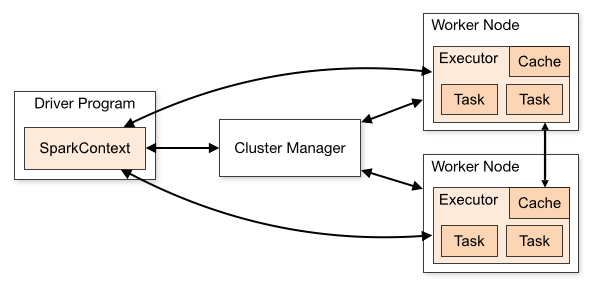
\includegraphics[scale=0.5]{pic/spark.png}
\end{figure}

A SparkContext is an interface between the Spark Driver Program
  (application) and the Spark runtime-system

\end{frame}



%-------------------------------------------------------------------
%-------------------------------------------------------------------
\begin{frame}[fragile]
\frametitle{WordCount Example in Spark}

\beb{Wordcount in Scala} 
\begin{code}
val lines = sc.textFile("hdfs://127.0.0.1:9000/input/")
val counts = lines.flatMap(line => line.split(" "))
    .map(word => (word, 1))
    .reduceByKey(_ + _)
counts.saveAsTextFile("hdfs://127.0.0.1:9000/output/")
\end{code} \eeb

\beb{Wordcount in Python}
\begin{code}
lines = sc.textFile("hdfs://127.0.0.1:9000/input/")
counts = lines.flatMap(lambda x: x.split(' ')) \
              .map(lambda x: (x, 1)) \
              .reduceByKey(add)
couts.saveAsTextFile("hdfs://127.0.0.1:9000/output/")
\end{code} \eeb
{\tt sc} denotes SparkContext 
\end{frame}




%-------------------------------------------------------------------
%-------------------------------------------------------------------
\begin{frame}[fragile]
\frametitle{WordCount Example in Spark}

\beb{Wordcount in Scala} 
\begin{code}
val lines:RDD[String] = 
    sc.textFile("hdfs://127.0.0.1:9000/input/")
val counts:RDD[(String,Long)] = 
    lines.flatMap(line => line.split(" "))
    .map(word => (word, 1))
    .reduceByKey(_ + _)
counts.saveAsTextFile("hdfs://127.0.0.1:9000/output/")
\end{code} \eeb
Recall in Scala {\tt  List(1,2,3).map( v => v + 1) }
yields  {\tt List(2,3,4) } \\ 
and {\tt List(List(1),List(2),List(3)).flatMap( l => l ) } 
yields
{\tt List(1,2,3) }
\\
An RDD can be seen as a distributed list. 
\end{frame}


%-------------------------------------------------------------------
%-------------------------------------------------------------------
\begin{frame}[fragile]
\frametitle{Resilient Distributed Dataset}

\begin{itemize} 
\item RDD is an abstraction over a collection of data set being distributed
and partitioned across a cluster of worker machines, mostly in memory.
\item Programmers are not required to manage or to coordinate that
distributed and partitioned. RDD is fault tolerant.  
\item RDDs are initialized and managed by the SparkContext.
\end{itemize}
\end{frame}




%-------------------------------------------------------------------
%-------------------------------------------------------------------


\begin{frame}[fragile]
\frametitle{RDD transformations are pure}

\begin{figure}[!htb]
\centering
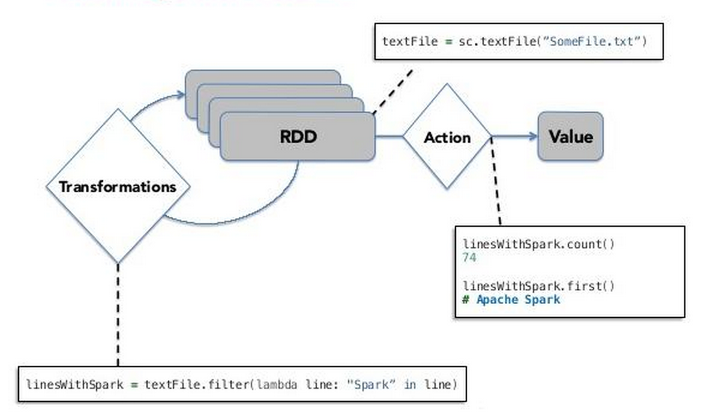
\includegraphics[scale=0.5]{pic/spark-rdd-partition-and-spark-rdd-architecture.png}
\end{figure}
Image adapted from {\tt http://www.hadooptpoint.com}

\end{frame}




%-------------------------------------------------------------------
%-------------------------------------------------------------------


\begin{frame}[fragile]
\frametitle{RDD transformations are pure}



Let {\tt r} denotes an RDD,
\begin{itemize}
\item {\tt r.map(f)} and {\tt r.flatMap(f)} applies {\tt f} to
  elements in {\tt r}.
\item {\tt r.filter(f)} filters away elements {\tt x} in {\tt r} which {\tt
    f(x)} yields {\tt false}.
\item assuming {\tt r} is a collection of key-value pairs, {\tt r.reduceByKey(f)} will
  shuffle the pairs and group them by keys. The values grouped under the same key will be
  reduced by {\tt f}. Data locality is exploit when possible.
\end{itemize}

\end{frame}



%-------------------------------------------------------------------
%-------------------------------------------------------------------


\begin{frame}[fragile]
\frametitle{RDD transformations are lazy}

\begin{itemize}
\item Computations do not take place unless the results are needed.
\item In memory cache are explicitly created.
\end{itemize}
\beb{Wordcount in Scala} 
\begin{code}
val lines:RDD[String] = 
    sc.textFile("hdfs://127.0.0.1:9000/input/")
val counts:RDD[(String,Long)] = 
    lines.flatMap(line => line.split(" "))
    .map(word => (word, 1))
    .reduceByKey(_ + _)
counts.persist() // caching
counts.saveAsTextFile("hdfs://127.0.0.1:9000/output/")
val somethingelse = counts.map( ... )
\end{code} \eeb

\end{frame}


%-------------------------------------------------------------------
%-------------------------------------------------------------------


\begin{frame}[fragile]
\frametitle{RDD transformations are resilient to node failure}

Since computations are pure, hence they are deterministic. 
Final results and intermediate results can be always recomputed.
\end{frame}





%-------------------------------------------------------------------
%-------------------------------------------------------------------



\begin{frame}[fragile]
\frametitle{How to run it?}

First start the cluster
\begin{code}
$ /opt/spark-1.4.1-bin-hadoop2.6/sbin/start-all.sh
\end{code}
%$
\end{frame}
%-------------------------------------------------------------------
%-------------------------------------------------------------------

\begin{frame}[fragile]
\frametitle{Run it in the REPL}

\beb{}
\begin{code}
$ /opt/spark-1.4.1-bin-hadoop2.6/bin/spark-shell
 scala> :load Wordcount.scala
\end{code}
%$
\eeb
Or we can type the code in line by line. 
\end{frame}


%-------------------------------------------------------------------
%-------------------------------------------------------------------

\begin{frame}[fragile]
\frametitle{Submit to the cluster}

\beb{Scala}
\begin{code}
$ /opt/spark-1.4.1-bin-hadoop2.6/bin/spark-submit
 Wordcount.jar
\end{code}
%$
\eeb

\beb{Python}
\begin{code}
$ /opt/spark-1.4.1-bin-hadoop2.6/bin/spark-submit 
wordcount.py
\end{code}
%$
\eeb

It supports R too.
\end{frame}


\end{document}
